\subsection{Matching}

Unter Matching eines Graphen versteht man eine Menge von Kanten von G, sodass keine zwei Kanten einen Knoten gemeinsam haben.

\begin{figure}[h]
\centering
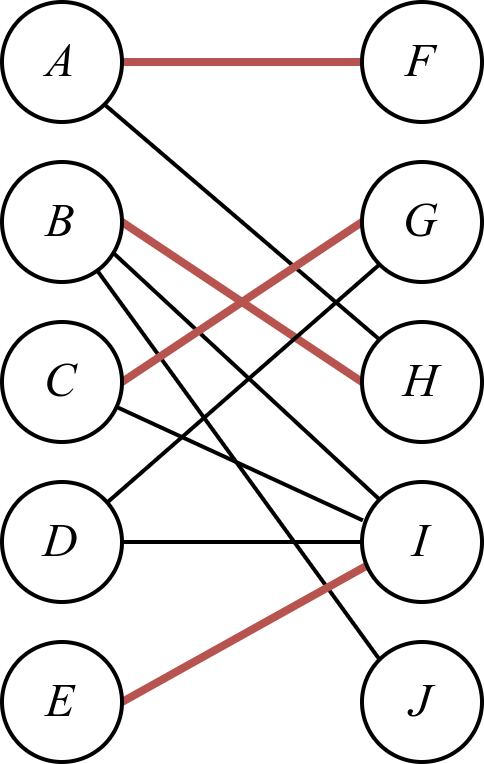
\includegraphics[width=0.2\textwidth]{graphics/graph_matching.png}
\end{figure}

$M = {(A,F), (B,H), (C,G), (E,I)}$ ist ein Matching der Mächtigkeit 4

\subsubsection*{Heiratssatz}

Im bipartiten Graphen $G = (S + T, E)$ gilt:

$$
m(G) = |S| \Leftrightarrow |A| \leq |N (A)| \text{ für alle } A \subseteq S
$$

\subsubsection*{Gesättigtes Matching}

Ein gesättigtes Matching ist ein Matching, bei dem man keinen Kante hinzufügen kann, ohne die Matching-Regeln verletzt werden.

\subsubsection*{Maximales Matching}

Ein maximales Matching in einem Graphen ist ein Matching, das die maximale/größtmögliche Anzahl von Kanten und Knotenpaare verbindet, ohne dass zwei Kanten einen Knoten gemeinsam haben. In einem Graph existiert also kein Matching, dass mehr Kanten hat als ein maximales Matching. Jedes maximales Matching ist somit auch ein gesättigtes  Matching.

\subsubsection*{Vollständiges Matching}

Ein vollständiges/perfektes Matching ist ein Matching, das alle Kanten des Graphen abdeckt, sodass jeder Knoten des Graphen mit genau einer Kante des Matchings verbunden ist.

\subsubsection*{Hopcraft-Karp Algorithmus}

